\documentclass[tikz]{standalone}
\usepackage{tikz}
\usepackage{graphicx}

\usetikzlibrary{calc, angles, quotes}
\usetikzlibrary{intersections} % Necessário para achar pontos de cruzamento

\begin{document}
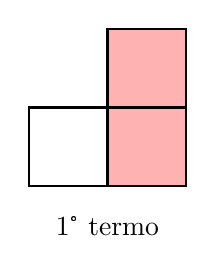
\begin{tikzpicture}
  \fill[red!30] (1,3) rectangle (2,5);    
  \foreach \x in {0,...,1} \draw[thick] (0+\x,3) rectangle (1+\x,4);
  \foreach \x in {1,...,1} \draw[thick] (0+\x,4) rectangle (1+\x,5);
  \node at (1,2.5) {$1$° termo};
\end{tikzpicture}

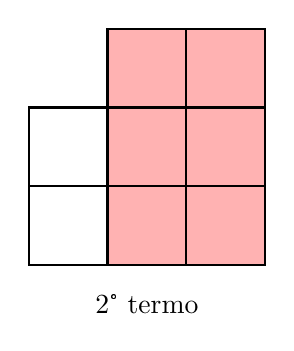
\begin{tikzpicture}
\fill[red!30] (1,2) rectangle (3,5);   
  \foreach \x in {0,...,2} \draw[thick] (0+\x,2) rectangle (1+\x,3);
  \foreach \x in {0,...,2} \draw[thick] (0+\x,3) rectangle (1+\x,4);
  \foreach \x in {1,...,2} \draw[thick] (0+\x,4) rectangle (1+\x,5);
  \node at (1.5,1.5) {$2$° termo};
\end{tikzpicture}

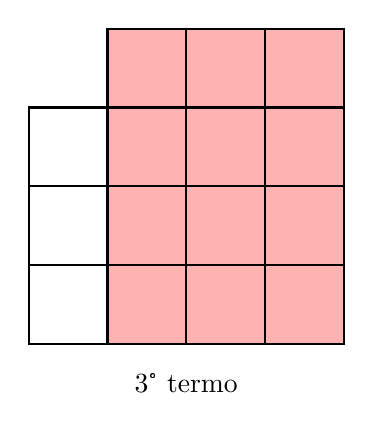
\begin{tikzpicture}
\fill[red!30] (1,1) rectangle (4,5);   
  \foreach \x in {0,...,3} \draw[thick] (0+\x,1) rectangle (1+\x,2);
  \foreach \x in {0,...,3} \draw[thick] (0+\x,2) rectangle (1+\x,3);
  \foreach \x in {0,...,3} \draw[thick] (0+\x,3) rectangle (1+\x,4);
  \foreach \x in {1,...,3} \draw[thick] (0+\x,4) rectangle (1+\x,5);
  \node at (2,.5) {$3$° termo};
\end{tikzpicture}
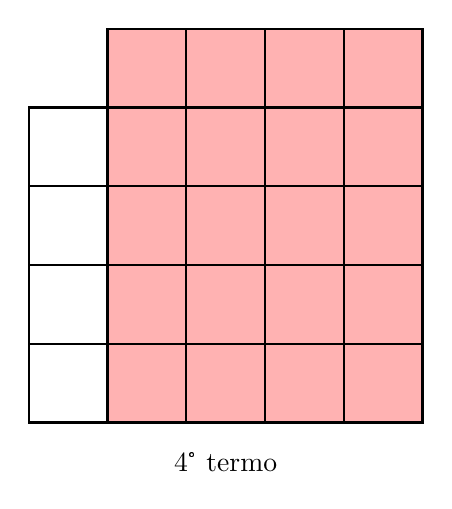
\begin{tikzpicture}
\fill[red!30] (1,0) rectangle (5,5);   
  \foreach \x in {0,...,4} \draw[thick] (0+\x,0) rectangle (1+\x,1);
  \foreach \x in {0,...,4} \draw[thick] (0+\x,1) rectangle (1+\x,2);
  \foreach \x in {0,...,4} \draw[thick] (0+\x,2) rectangle (1+\x,3);
  \foreach \x in {0,...,4} \draw[thick] (0+\x,3) rectangle (1+\x,4);
  \foreach \x in {1,...,4} \draw[thick] (0+\x,4) rectangle (1+\x,5);
  \node at (2.5,-.5) {$4$° termo};
\end{tikzpicture}
\end{document}